\begin{table*}
    \begin{minipage}[b]{0.6\linewidth}
        \centering
    \small
    \captionof{table}{
    Needle-In-A-Haystack experiments with: (1) Single needle with three levels of difficulty: single-needle tasks—S-NIAH-1 (passkey retrieval), S-NIAH-2 (numerical needle), and S-NIAH-3 (UUID-based needle); (2) multi-query; (3) multi-key; and (4) multi-value settings of the benchmark.} \label{tab:ruler}
    \hspace{3ex}
    \resizebox{\linewidth}{!}{
    \begin{tabular}{lccccccccc}
    \toprule
     & \multicolumn{3}{c}{\textbf{S-NIAH-1}}  & \multicolumn{3}{c}{\textbf{S-NIAH-2}} & \multicolumn{3}{c}{\textbf{S-NIAH-3}}  \\
    & \multicolumn{3}{c}{(pass-key retrieval)} & \multicolumn{3}{c}{(number in haystack)} & \multicolumn{3}{c}{(uuid in haystack)}  \\
    \cmidrule(lr){2-4} \cmidrule(lr){5-7} \cmidrule(lr){8-10}
    \textbf{Model}  & 4K  & 8K & 16K & 4K & 8K & 16K & 4K & 8K & 16K  \\
    \midrule
    Transformer          &  88.6 & 76.4 & 79.8 & 100 & 98.8 & 94.2 & 78.0 & 69.2 & 40.8 \\
    \rowcolor{mygray} \model-Attention & 100 & 100 & 100 & 100 & 98.4 & 94.4 & 76.8 & 68.8 & 42.4 \\
    \midrule
    RWKV-7 & 100 & 100 & 99.6 & 93.8 & 44.8 & 12.6 & 63.8 & 13.2 & 5.8\\
    Comba & 100 & 100 & 99.4  & 92.6 & 47.2 & 13.4 & 62.4 & 13.8 & 7.4\\
    DLA             & 96.4 & 71.2 & 44.0 & 79.6 & 42.6 & 28.2 & 18.2 & 8.8 & 4.0 \\
    Titans      & 100 & 100 & 100 & 99.6 & 84.6 & 75.4 & 74.2 & 42.8 & 21.2 \\
    \midrule
    \rowcolor{mygray}\model & 100 & 100 & 100 & 99.2 & 88.4 & 78.2 & 73.2 & 46.2 & 24.8 \\
    \toprule
    \addlinespace
    & \multicolumn{3}{c}{\textbf{MK-NIAH-1}} & \multicolumn{3}{c}{\textbf{MQ-NIAH}}& \multicolumn{3}{c}{\textbf{MV-NIAH}} \\
    & \multicolumn{3}{c}{(multi-key line retrieval)} & \multicolumn{3}{c}{(multi-query)} & \multicolumn{3}{c}{(multi-value)}  \\
    \cmidrule(lr){2-4} \cmidrule(lr){5-7} \cmidrule(lr){8-10}
    \textbf{Model}  & 4K & 8K & 16K & 4K & 8K & 16K & 4K & 8K & 16K  \\
    \midrule
    Transformer      & 79.4 & 83.0 & 61.4 & 58.9 & 48.0 & 29.8 & 37.5 & 34.1 & 21.5 \\
    \rowcolor{mygray} \model-Attention & 80.2 & 84.8 & 60.8 & 60.4 & 47.8 & 30.6 & 35.2 & 34.4 & 24.8 \\
    \midrule
    RWKV-7 & 21.4   & 18.8  &  9.6    &  20.4  & 14.8  &  8.6  & 16.2 & 13.4 & 6.8\\
    Comba &  21.4   & 19.4  &   8.2   &  21.8  & 15.2  &  6.4  & 16.5 & 13.5   & 7.2 \\
    DLA             & 27.4 & 20.0 & 11.8 & 26.4 & 22.0 & 6.4 & 25.6 & 12.8 & 9.6 \\
    Titans       & 26.4 & 23.6 & 8.2 & 22.8 & 19.8 & 9.4 & 24.6 & 15.1 & 8.2 \\
    \midrule
    \rowcolor{mygray}\model & 29.4 & 24.8 &  14.8 & 31.7  & 24.8 & 14.2 & 31.4 & 17.2 & 11.4 \\
    \bottomrule
    \end{tabular}
    }
    \centering
    \end{minipage}~\hspace{1ex}~
    \begin{minipage}{0.37\linewidth}
            \begin{minipage}{\linewidth}
                \centering
                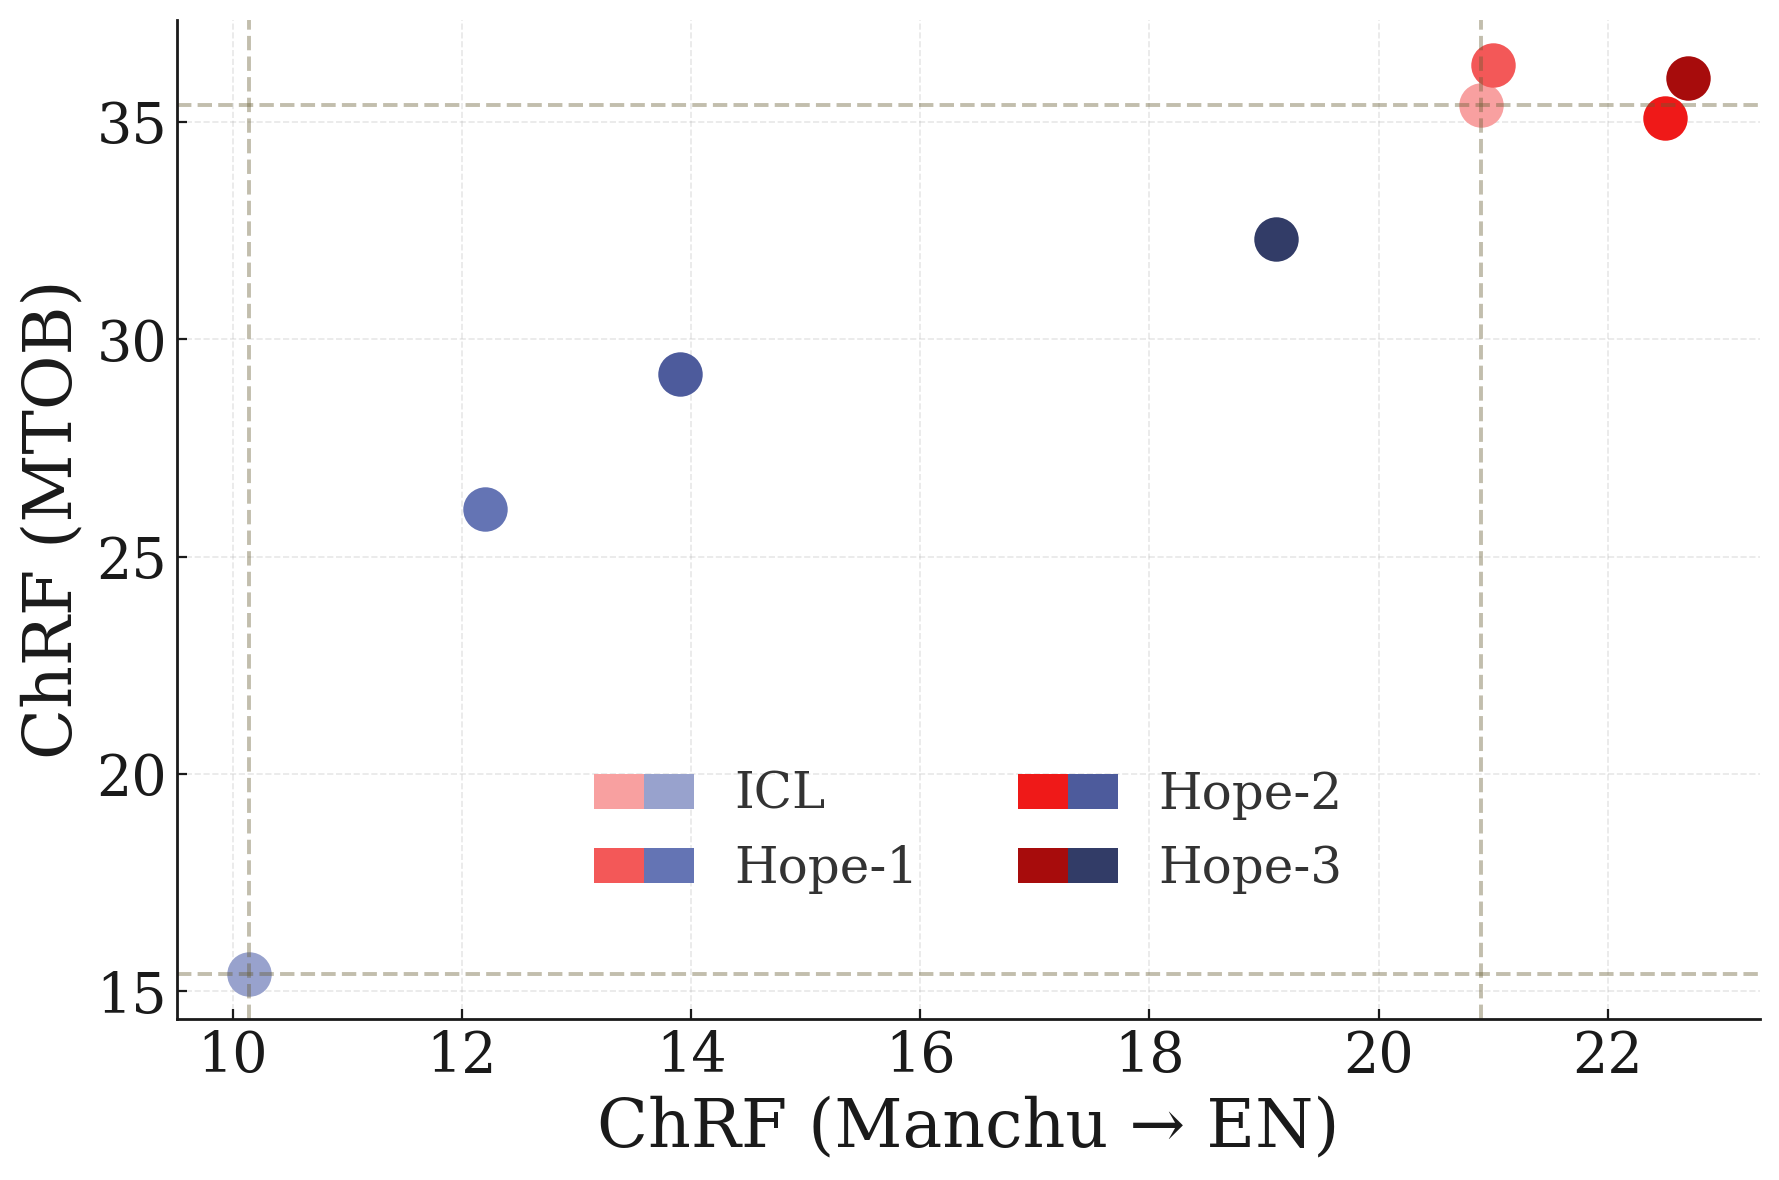
\includegraphics[width=\linewidth]{Images/ICL-Translate.png}
                \captionof{figure}{Continual Translation of a Novel Language (CTNL) task. \textcolor{darkred}{Red} points are the results with only one language.  \textcolor{darkblue}{Blue} points are the results in the continual leanring setup.}
                \label{fig:icl-translate}
            \end{minipage}
            \vspace*{10ex}
            \begin{minipage}{\linewidth}
                \centering
                \vspace{1ex}
                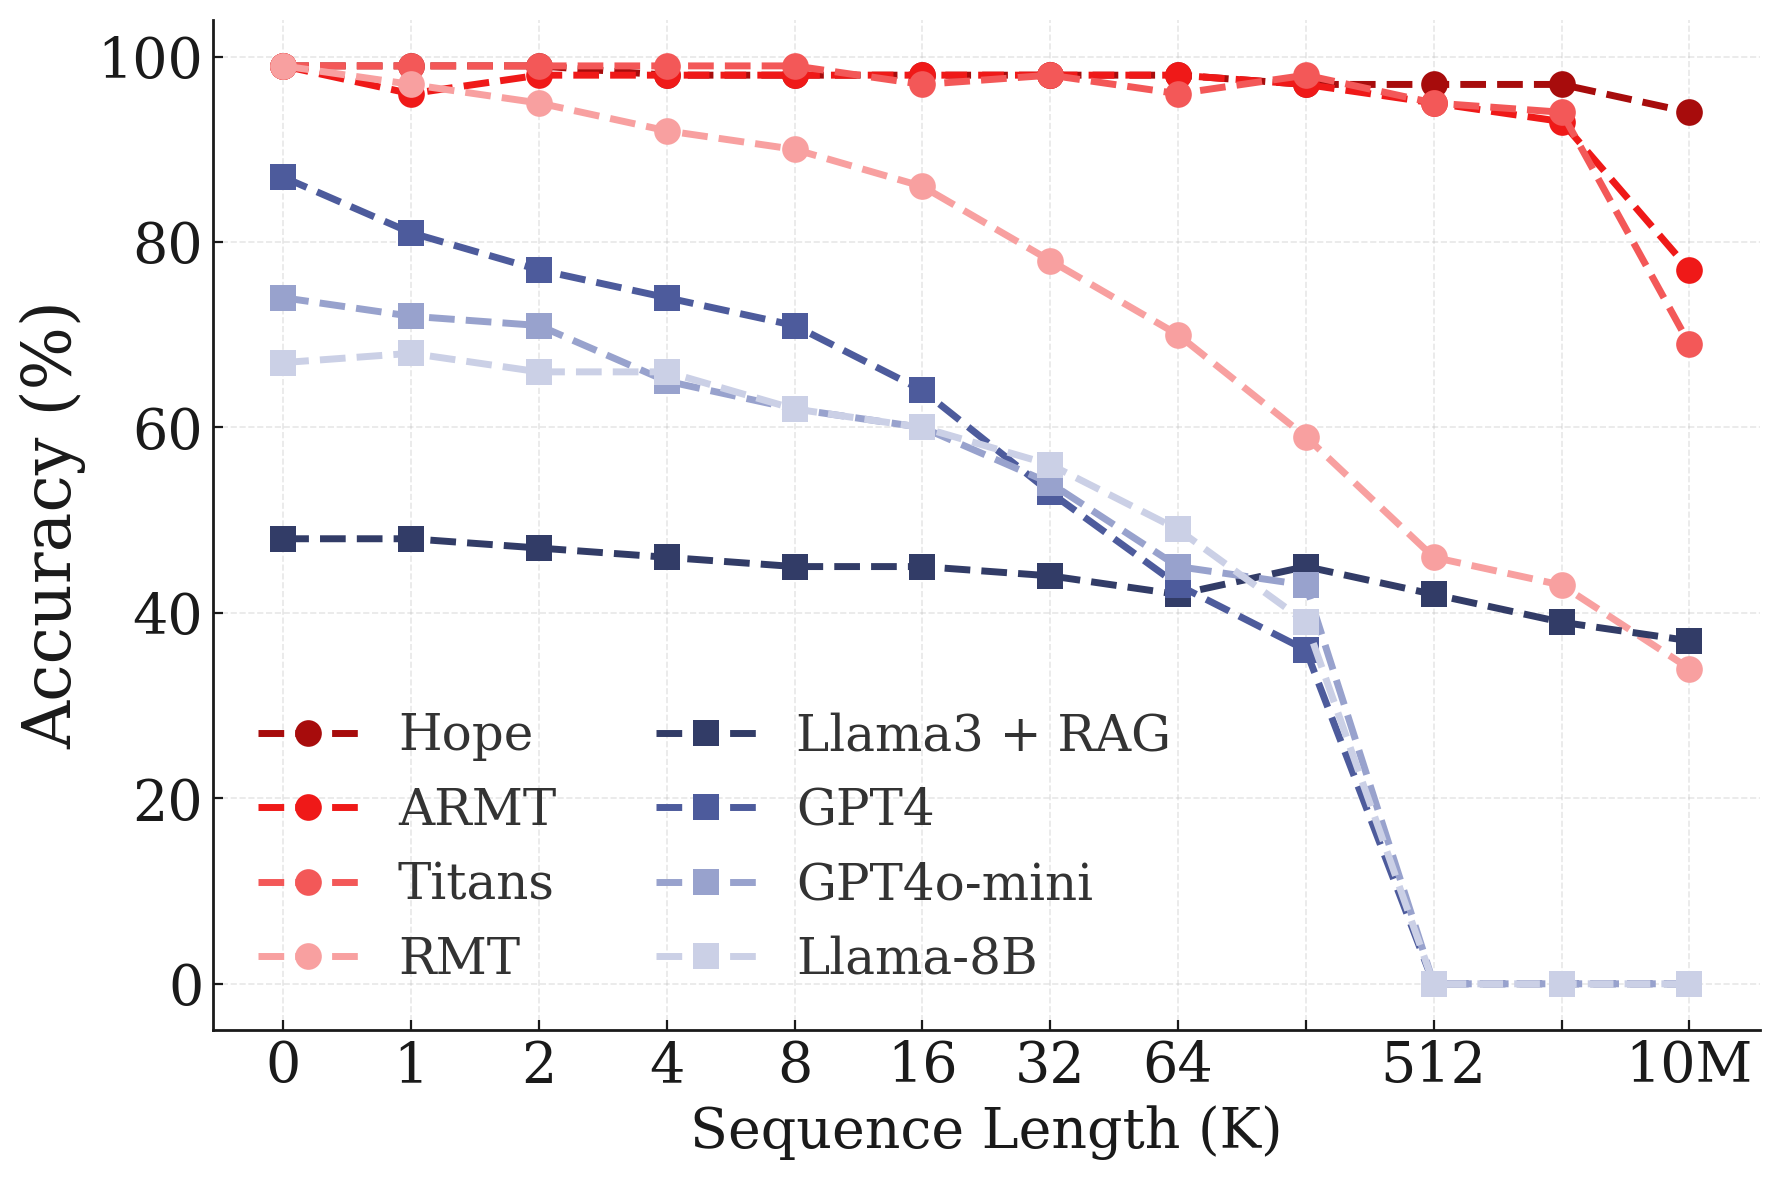
\includegraphics[width=\linewidth]{Images/BABILong.png}
                \captionof{figure}{BABILong Benchmark. \textcolor{darkred}{Red} points are the results of fine-tuned models, and \textcolor{darkblue}{Blue} points are the large models' zero-shot results. }
                \label{fig:babilong}
                \vspace{-7ex}
            \end{minipage}
    \end{minipage}
\end{table*}